\documentclass[12pt]{article}

\usepackage[T2A]{fontenc}
\usepackage[utf8]{inputenc}
\usepackage[english,russian]{babel}

\usepackage[T2A]{fontenc}
\usepackage[utf8]{inputenc}
\usepackage[russian]{babel}

\usepackage[
    a4paper,
    left=3cm,
    right=2cm,
    top=2cm,
    bottom=2cm
]{geometry}

%% Figures
\usepackage{tkz-euclide}
\usepackage{subcaption}
\usepackage{amsmath}
\usepackage{amssymb}

%% Hyphenation rules
\usepackage{hyphenat}

\usepackage[hidelinks]{hyperref}

%%colorfull
\usepackage{xcolor}

\usepackage{indentfirst}

\usepackage{graphicx}

\DeclareGraphicsExtensions{.pdf,.png,.jpg}
\graphicspath{ {pic/} }
% Настройка списков
\usepackage{enumitem}
\setlist{nolistsep, labelsep=0.4cm, leftmargin=1.85cm}

% Красная строка у первого абзаца посе заголовка
% (по умолчанию не ставится)
\usepackage{indentfirst}

\begin{document}
\begin{figure}[h!]
    \centering
    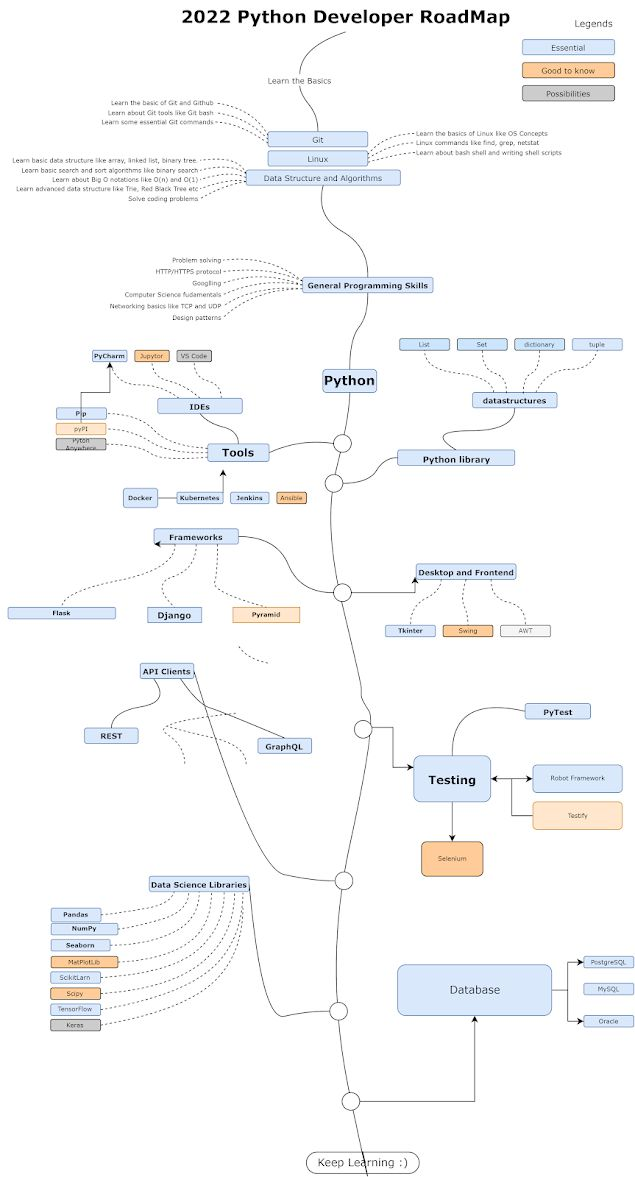
\includegraphics[width=\textwidth,height=0.97\textheight,keepaspectratio]{10-2-1}
    \caption{\small Python roadmap}
\end{figure}
\end{document}